\section{Vector Processing and Computing $\pi$}

The PAPI measurements were added only around the core computation regions.
For vector addition, the measured region is the OpenMP loop that computes
\texttt{a[i] = b[i] + c[i]}. For the $\pi$ program, the measured region is the
OpenMP reduction loop. Memory allocation, initialization, and printing are not
included in the measured regions.

The counters \texttt{PAPI\_VEC\_SP} and \texttt{PAPI\_VEC\_DP} were tested, but
they were not available on the assigned machine, so the corresponding values
are not reported.

\subsection{Vector Addition}

\begin{table}[H]
\centering
\resizebox{\textwidth}{!}{
\begin{tabular}{r|r|r|r|r|r|r|r}
\hline
Threads & Size & Time (s) & L1-I Misses & L1-D Misses & L2 Misses & \# instructions & \# cycles \\
\hline
1  & 100000000 & 0.897026418 & 6346  & 14284687 & 902659  & 600195806  & 1370172736 \\
2  & 100000000 & 0.460777812 & 5784  & 14443166 & 865054  & 602296050  & 1234609617 \\
4  & 100000000 & 0.299388644 & 5484  & 14345967 & 799188  & 606496666  & 1618929973 \\
8  & 100000000 & 0.229260495 & 15714 & 14439129 & 2498055 & 614897837  & 2194077522 \\
16 & 100000000 & 0.219199555 & 10995 & 14353115 & 6630137 & 631700378  & 2996526759 \\
\hline
\end{tabular}}
\caption{Vector addition behavior for size $10^8$}
\label{tab:vector-papi-1e8}
\end{table}

\begin{figure}[H]
\centering
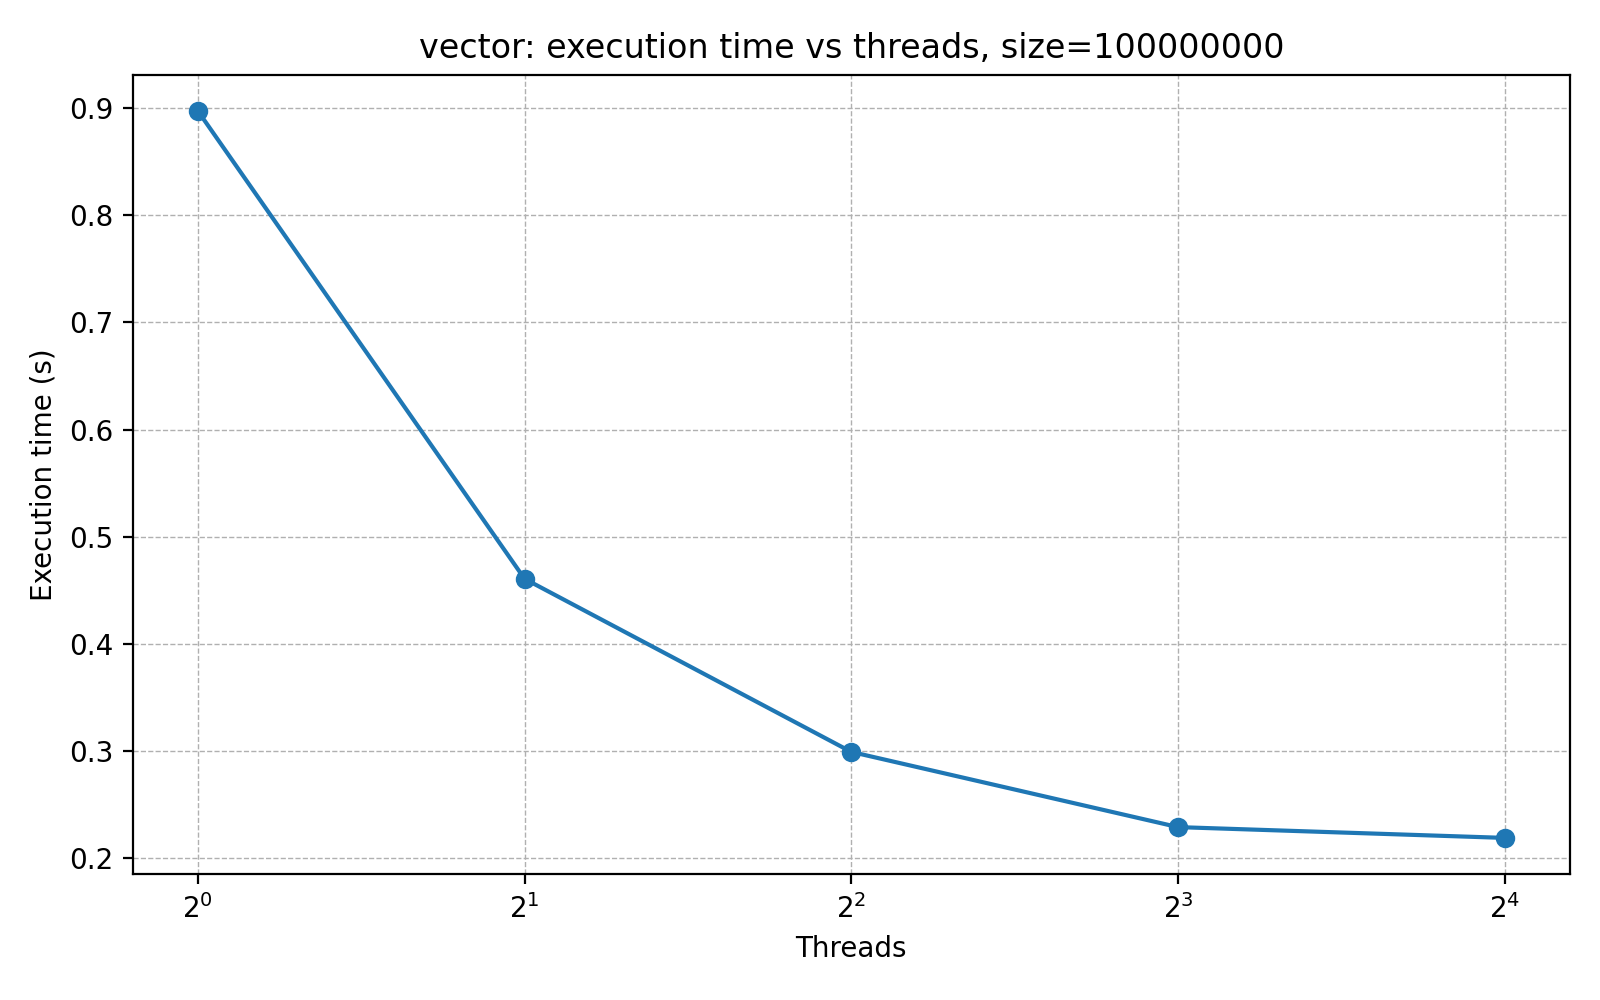
\includegraphics[width=0.72\textwidth]{vector_time_vs_threads.png}
\caption{Vector addition execution time vs. threads for size $10^8$}
\label{fig:vector-time-threads}
\end{figure}

\begin{figure}[H]
\centering
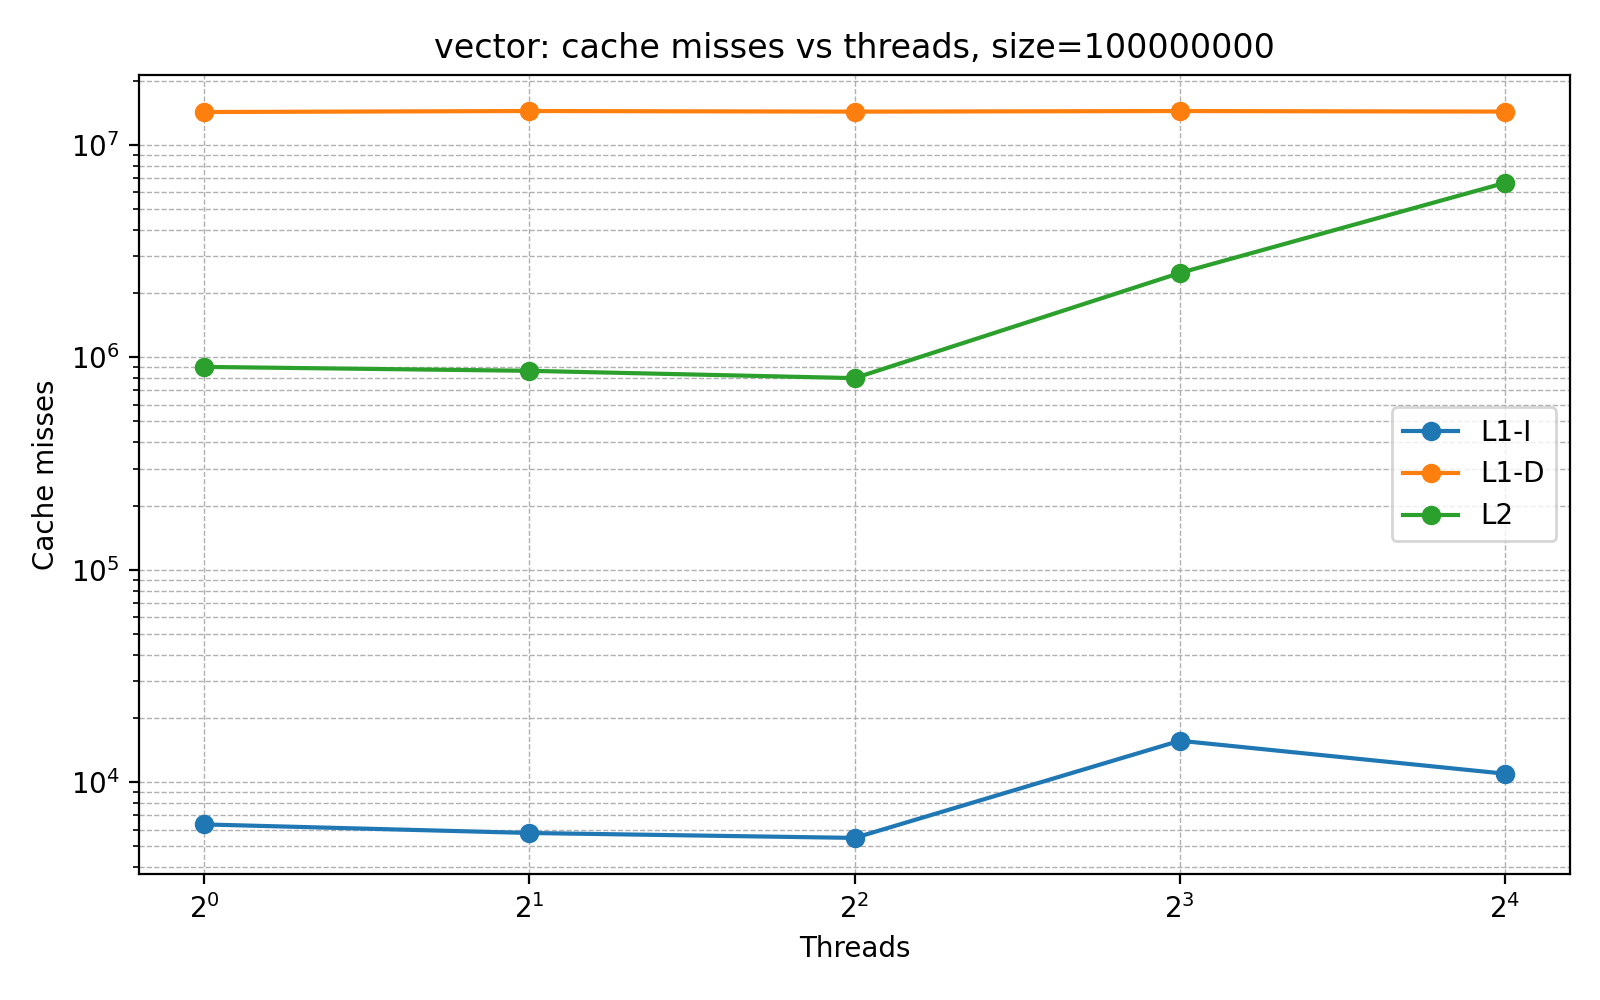
\includegraphics[width=0.72\textwidth]{vector_misses_vs_threads.png}
\caption{Vector addition cache misses vs. threads for size $10^8$}
\label{fig:vector-misses-threads}
\end{figure}

\subsection{Computing $\pi$}

\begin{table}[H]
\centering
\resizebox{\textwidth}{!}{
\begin{tabular}{r|r|r|r|r|r|r|r}
\hline
Threads & Size & Time (s) & L1-I Misses & L1-D Misses & L2 Misses & \# instructions & \# cycles \\
\hline
1  & 100000000 & 0.361157580 & 727  & 407  & 173 & 1200000551 & 1092586146 \\
2  & 100000000 & 0.184191758 & 281  & 472  & 249 & 1202100752 & 1070365936 \\
4  & 100000000 & 0.165281171 & 831  & 614  & 471 & 1206301513 & 1501818962 \\
8  & 100000000 & 0.091561853 & 1306 & 1123 & 485 & 1212832602 & 1610017289 \\
16 & 100000000 & 0.060157154 & 1780 & 2007 & 965 & 1231504969 & 2001735387 \\
\hline
\end{tabular}}
\caption{Computing $\pi$ behavior for size $10^8$}
\label{tab:pi-papi-1e8}
\end{table}

\begin{figure}[H]
\centering
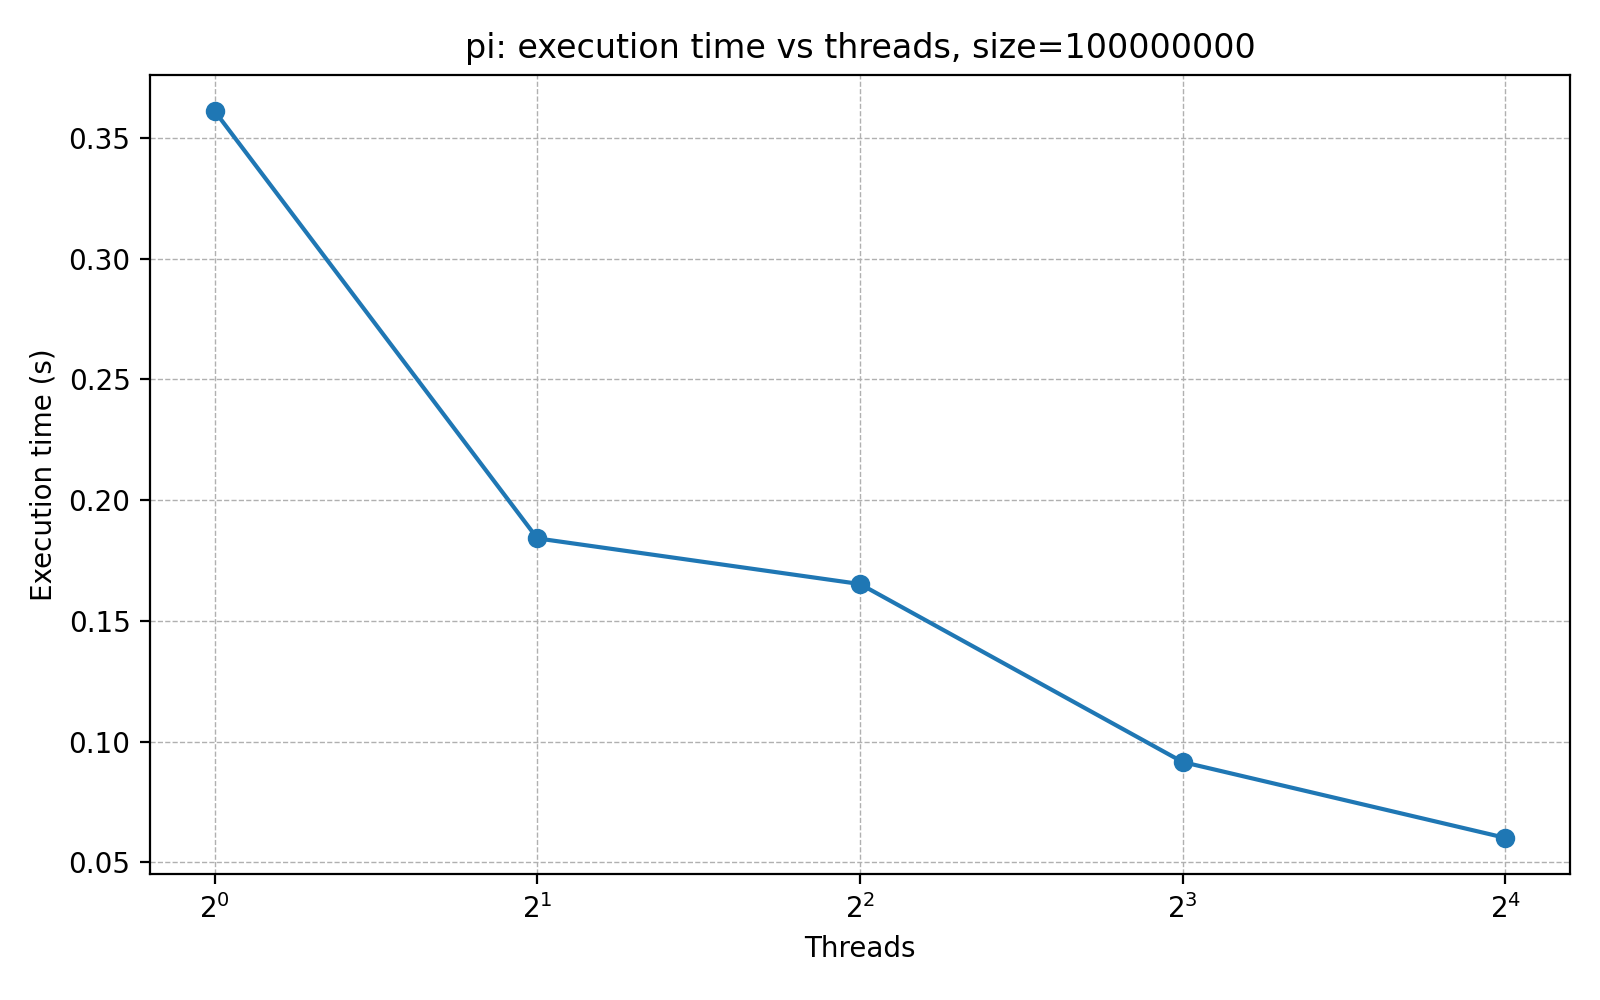
\includegraphics[width=0.72\textwidth]{pi_time_vs_threads.png}
\caption{Computing $\pi$ execution time vs. threads for size $10^8$}
\label{fig:pi-time-threads}
\end{figure}

\begin{figure}[H]
\centering
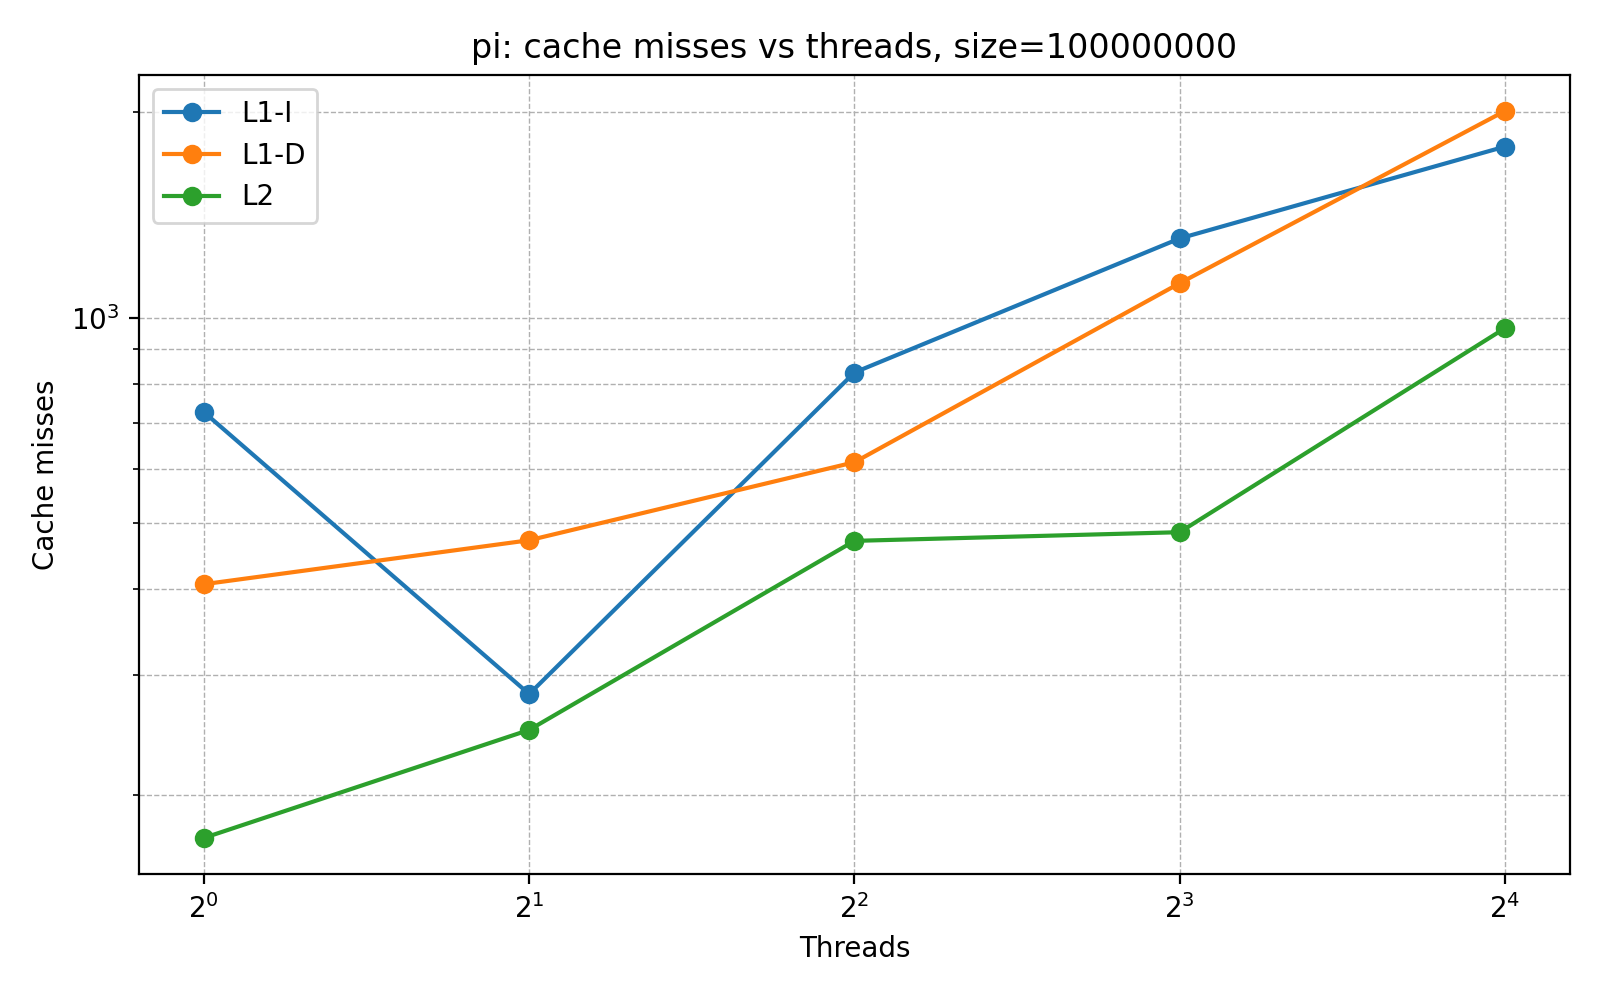
\includegraphics[width=0.72\textwidth]{pi_misses_vs_threads.png}
\caption{Computing $\pi$ cache misses vs. threads for size $10^8$}
\label{fig:pi-misses-threads}
\end{figure}

\subsection{Questions}

\begin{enumerate}
    \item \textbf{Can performance degradation be explained by cache behavior?}

    For vector addition, cache behavior explains part of the performance trend.
    The execution time improves as the number of threads increases, but the
    improvement becomes smaller at higher thread counts. At size $10^8$, time
    decreases from 0.897 s with 1 thread to 0.219 s with 16 threads, while L2
    misses increase from 902,659 to 6,630,137. This suggests that cache effects
    become more visible at high thread counts and may limit scaling.

    For the $\pi$ computation, cache behavior is less important. The data
    footprint is very small, and L1-D/L2 misses remain much lower than in vector
    addition. Performance is mainly related to computation, not memory traffic.

    \item \textbf{Which cache level has the strongest impact on performance?}

    For vector addition, L2 behavior appears to have the strongest impact among
    the measured cache levels. L1-D misses are already high because the program
    streams through large arrays, but the large increase in L2 misses at 8 and
    16 threads is more closely associated with the reduced scaling. For example,
    L2 misses increase from 799,188 with 4 threads to 2,498,055 with 8 threads
    and 6,630,137 with 16 threads.

    For the $\pi$ computation, no cache level has a strong visible impact,
    because the kernel mostly operates on scalar local variables and does not
    stream through large arrays.

    \item \textbf{Is cache coherence affecting the performance?}

    There is no strong evidence that cache coherence is the main factor. The
    original cache-coherence events requested in the assignment were not
    available on the machine, so they could not be measured directly. From the
    program structure, vector addition assigns different array elements to
    different threads, and the $\pi$ program uses a reduction. These patterns do
    not create heavy shared writes to the same cache lines in the core loop.
    Therefore, cache coherence may add some overhead, but it does not appear to
    dominate performance.

    \item \textbf{Is the application memory-bound or compute-bound?}

    Vector addition is more memory-bound. Each iteration performs very little
    arithmetic but reads two arrays and writes one array, so performance depends
    heavily on moving data through the memory hierarchy. This is consistent with
    the relatively large L1-D and L2 miss counts.

    The $\pi$ computation is more compute-bound. It performs floating-point
    arithmetic in each iteration and uses only a few scalar variables. Its cache
    miss counts are much smaller, so memory traffic is not the main bottleneck.
\end{enumerate}
